\chapter{Pian cu temporizator 555}
\section{Descrierea componentelor}

\vspace{5mm}
Schema circuitului cuprinde: 
\begin{enumerate}
\color{blue}
\item 12 butoane
\item 9 rezistoare de 1$K\Omega$
\item 3 rezistoare de 2$K\Omega$
\item 1 rezistor de 6,2$K\Omega$
\item 1 condensator de 100 $nF$
\item 1 baterie de 9V si 25 $\Omega$
\item 1 temporizator 555
\item 1 difuzor
\item 2 t'abli'te Breadboard
\item 52 de fire de dimensiuni diferite
\end{enumerate}

\vspace{5mm}
\myindent
\textbf{Temporizatorul 555} reprezint'a un cip folosit cu scopul de a crea impulsuri de durate diferite pentru a crea o form'a de und'a continu'a 'intre st'arile joase sau 'inalte. Temporizatorul 555 este foarte flexibil, ieftin 'si usor de g'asit, ceea ce il face o pies'a de circuit cu un punct de plecare favorabil pentru proiecte mici precum : ceasuri sau proiecte audio. Ata's\^and dispozitivului rezisten'te 'si condensatori 'in diferite moduri se pot ob'tine 3 moduri diferite de func'tionare:

\vspace{5mm}
\begin{enumerate}
\color{violet}
\item \textbf{Modul Monostabil} - folosit pentru a crea 'int\^arzieri. 'In acest mod, un declan'sator extern face ca cipul s'a emit'a un impuls de o durat'a reglabil'a
\item \textbf{Modul Astable} - emite un semnal sub form'a de und'a, cipul comut'a 'intre st'arile 'inalte 'si joase la o frecven't'a reglabil'a
\item \textbf{Modul Bistabil} - comut'a 'intre st'arile 'inalte 'si joase, dar pentru dou'a intr'ari 
\end{enumerate}

\section{Descrierea circuitului}
\myindent
Schema pianului folose'ste temporizatorul 555 'in modul Astable, deoarece fiecare not'a are o frecven't'a principal'a, drept pentru care, prin manipularea frecven'tei se pot ob'tine sunete diferite. Frecven'ta produs'a de temporizator se bazeaz'a pe valorile condensatorului 'si a celor dou'a rezistente R1 'si R2, unde R1 este rezisten'ta dintre pin-ul \textbf{Discharge} al temporizatorului 'si borna pozitiv'a a bateriei, iar R2 este rezisten'ta echivalent'a a rezistoarelor care sunt parcurse de la pin-ul \textbf{Discharge} al temporizatorului 'si butonul care este ap'asat. 'In cazul 'in care sunt ap'asate mai multe butoane deodat'a, curentul va parcurge circuitul p\^an'a la butonul care are rezisten'ta echivalent'a R2 mai mic'a.

\vspace{5mm}
\myindent
Formula care determin'a frecven'ta de ie'sire a circuitului este: \\
\[ frecventa = \frac{1}{7(R1+R2)C}\]\\

\section{Link-uri 'si scheme}
\myindent
Link-ul circuitului: \url{https://www.tinkercad.com/things/kGCP1YdP2NQ}

\vspace{10mm}
\begin{figure}[ht]
\centering
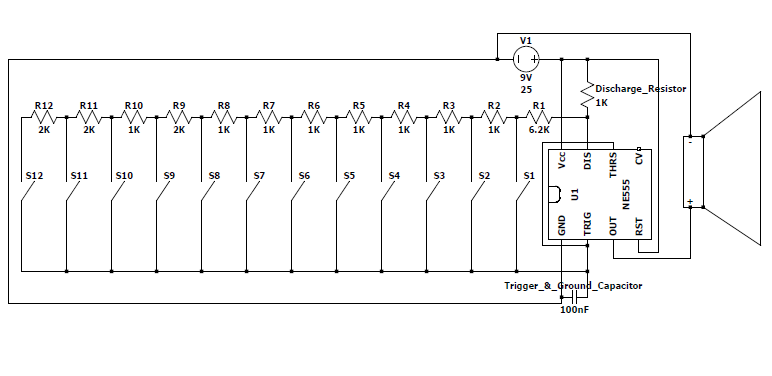
\includegraphics[scale=0.8]{Fisiere/Schema}
\caption {Schema circuitului implementat'a in LTSpice}
\end{figure}
\FloatBarrier

